%!TEX root = ../Master.tex

\section{SLAM}

A fundamental problem involved with AI in robotics is localization and mapping. This problem arise when the robot does not have a map of the environment and do not know it's pose. Usually the only information the robot have at it's disposal is measurement and control-inputs. This problem is commonly referred to as \textit{Simultaneous Localization And Mapping} abbreviated as \textit{SLAM}.\\

A technique to solve the SLAM problem is called GraphSLAM. As the name suggest, this technique represents the robots poses and landmarks as nodes in a graph and constraints between poses, resulting from measurements, are encoded on the edges between nodes. An edge between two nodes therefore represents a spatial constraint relating the two robot poses. Since constraints are generated from measurements which we represent as Gaussians because of measurement uncertainty, the goal then, is to find a configuration of the nodes that minimize the error introduced by the constraints.\\

We represent the constraints between poses and landmarks using a matrix $\Omega$ and a vector $\xi$. The matrix describes which object (poses and landmarks) in the environment that are related, and the vector contains a value for this relationship which could be a distance between the objects. When new constraint are generated by the robot, the matrix and vector is modified by added the constraints to a subset of the matrix and vector.\\

Once the constraints have been defined in the matrix and vector pair, the best estimate of the robot poses and landmarks positions can be calculated by inverting the matrix $\Omega$ and multiplying it with vector $\xi$ as giving by Equation \ref{eq:slam_est}.

\begin{equation}
\label{eq:slam_est}
\mu = \Omega^{-1}\xi
\end{equation}

To summarize, in the graph-based SLAM technique, we add information to the matrix $\Omega$ and vector $\xi$ every time an constraint is encountered, and when we are done gathering constraints a simple procedure is run which gives the robot poses and landmark locations.

\subsection{GraphSLAM example}

In this section a simple example is giving on how to use GraphSLAM which involves defining constraints and solving a system of equations to obtain robot and landmark locations.\\

Giving the graph in \autoref{fig:slam_ex} which shows three robot poses and a landmark, we need a matrix of size $4\times4$ and a vector of size 4 to describe all the constraints. The initial position of the robots is $x_0 = -3$ and we can define the local constraints of movement $x_0 \rightarrow x_1$ and $x_1 \rightarrow x_2$ as Equation \ref{eq:slam_pose_rel1_a} and \ref{eq:slam_pose_rel1_b}, respectively.

\begin{equation}
\label{eq:slam_pose_rel1_a}
x_1 = x_0 + 5
\end{equation}

\begin{equation}
\label{eq:slam_pose_rel1_b}
x_2 = x_1 + 3
\end{equation}

Which gives constraints in Equation \ref{eq:slam_pose_rel2_a} - \ref{eq:slam_pose_rel3_b}.

\begin{equation}
\label{eq:slam_pose_rel2_a}
x_0 - x_1 = -5
\end{equation}

\begin{equation}
\label{eq:slam_pose_rel2_b}
x_1 - x_0 = 5
\end{equation}

\begin{equation}
\label{eq:slam_pose_rel3_a}
x_1 - x_2 = -3
\end{equation}

\begin{equation}
\label{eq:slam_pose_rel3_b}
x_2 - x_1 = 3
\end{equation}

Adding constraints in Equation \ref{eq:slam_pose_rel2_a} and \ref{eq:slam_pose_rel2_b} together with the initial position of the robot, gives the matrix and vector shown in Equation \ref{eq:slam_matrix1}.

\begin{equation}
\label{eq:slam_matrix1}
\begin{bmatrix}
2 & -1 & 0 & 0 \\
-1 & 1 & 0 & 0 \\
0 & 0 & 0 & 0 \\
0 & 0 & 0 & 0 \\
\end{bmatrix}
\begin{bmatrix}
-8 \\
5 \\
0 \\
0 \\
\end{bmatrix}
\end{equation}

Adding the constraint relating $x_1$ to $x_2$ results in the matrix and vector shown in Equation \ref{eq:slam_matrix2}.

\begin{equation}
\label{eq:slam_matrix2}
\begin{bmatrix}
2 & -1 & 0 & 0 \\
-1 & 2 & -1 & 0 \\
0 & -1 & 1 & 0 \\
0 & 0 & 0 & 0 \\
\end{bmatrix}
\begin{bmatrix}
-8 \\
2 \\
3 \\
0 \\
\end{bmatrix}
\end{equation}

Now we need to add the constraints relating the robot poses to the landmark.

\begin{figure}[H]
\centering
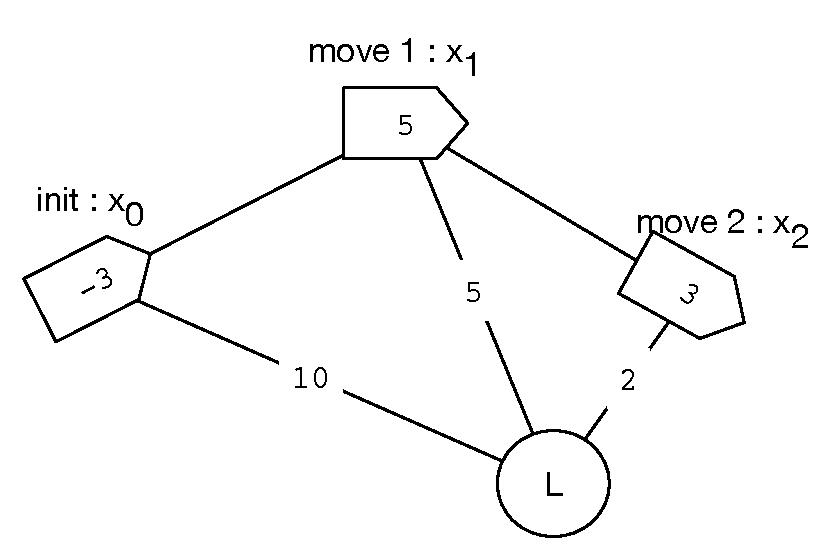
\includegraphics[scale=0.70]{images/ex_slam_graph}
\caption{GraphSLAM example}
\label{fig:slam_ex}
\end{figure}

The relation between the three poses and the landmark is giving by Equation \ref{eq:slam_lan_rel1} - \ref{eq:slam_lan_rel3}.

\begin{equation}
\label{eq:slam_lan_rel1}
L = x_0 + 10
\end{equation}

\begin{equation}
\label{eq:slam_lan_rel2}
L = x_1 + 5
\end{equation}

\begin{equation}
\label{eq:slam_lan_rel3}
L = x_2 + 2
\end{equation}

Which gives the constraints for $x_0 \rightarrow L$.

\begin{equation}
\label{eq:slam_lan_cons1_a}
x_0 - L = -10
\end{equation}

\begin{equation}
\label{eq:slam_lan_cons1_b}
L - x_0 = 10
\end{equation}

And for $x_1 \rightarrow L$.

\begin{equation}
\label{eq:slam_lan_cons2_a}
x_1 - L = -5
\end{equation}

\begin{equation}
\label{eq:slam_lan_cons2_b}
L - x_1 = 5
\end{equation}

And lastly for $x_2 \rightarrow L$.

\begin{equation}
\label{eq:slam_lan_cons3_a}
x_2 - L = -2
\end{equation}

\begin{equation}
\label{eq:slam_lan_cons3_b}
L - x_2 = 2
\end{equation}

Adding these constraints to the matrix and vector in Equation \ref{eq:slam_matrix2} produces the matrix and vector in Equation \ref{eq:slam_matrix3}.

\begin{equation}
\Omega =
\label{eq:slam_matrix3}
\begin{bmatrix}
3 & -1 & 0 & -1 \\
-1 & 3 & -1 & -1 \\
0 & -1 & 2 & -1 \\
-1 & -1 & -1 & 3 \\
\end{bmatrix}\,
\xi =
\begin{bmatrix}
-18 \\
-3 \\
1 \\
17 \\
\end{bmatrix}
\end{equation}

Solving this system using Equation \ref{eq:slam_est} produces the best estimate $\mu$ shown in Equation \ref{eq:slam_calc}.

\begin{equation}
\label{eq:slam_calc}
\mu = \Omega^{-1}\xi = 
\begin{bmatrix}[2.2]
1 & 1 & 1 & 1 \\
1 & \dfrac{13}{8} & \dfrac{3}{2} & \dfrac{11}{8} \\
1 & \dfrac{3}{2} & 2 & \dfrac{3}{2} \\
1 & \dfrac{11}{8} & \dfrac{3}{2} & \dfrac{13}{8} \\
\end{bmatrix}
\begin{bmatrix}[2.2]
-18 \\
-3 \\
1 \\
17 \\
\end{bmatrix} =
\begin{bmatrix}[2.2]
-3 \\
2 \\
5 \\
7 \\
\end{bmatrix}
\end{equation}

Meaning that the positions of the robot and the landmark are $x_0 = -3$, $x_1 = 2$, $x_2 = 5$, and $L = 7$. Note that in Equation \ref{eq:slam_matrix3} matrix $\Omega$ has zeros in positions $\Omega_{3,1}$ and $\Omega_{1,3}$ meaning that there is no constraint between $x_0$ and $x_2$. This can also be seen in \autoref{fig:slam_ex} because there is no edge between these two nodes.

